%\documentclass[twocolumn]{article}
\documentclass[twocolumn,apj]{aastex63}
\pdfoutput=1
\usepackage{amsmath,amssymb,gensymb,color,graphicx,array,multirow,soul,rotating}
\usepackage{natbib,multirow,placeins,textcomp,subfigure}
\usepackage[outline]{contour}
%\usepackage[margin=14mm,top=10mm]{geometry}
\usepackage[utf8]{inputenc}
\usepackage[T1]{fontenc}
%\usepackage{threeparttable}
\usepackage{booktabs}
\usepackage{microtype}
%\usepackage{bm}
\usepackage{listings}
\usepackage{hyperref}
\usepackage{savesym}
\savesymbol{splitbox}
\usepackage[export]{adjustbox}

\newcommand{\planck}{{\it Planck}}
\newcommand{\wmap}{{\sl WMAP}}
\newcommand{\cobe}{{\sl COBE}}
\newcommand{\code}[1]{\texttt{#1}}
\newcommand{\vc}[1]{\begin{minipage}[c]{\linewidth}{\begin{center}#1\end{center}}\end{minipage}}

\newcolumntype{C}[1]{>{\centering\arraybackslash}m{#1}}

\DeclareFixedFont{\ttb}{T1}{txtt}{bx}{n}{9} % for bold
\DeclareFixedFont{\ttm}{T1}{txtt}{m}{n}{9}  % for normal
\DeclareRobustCommand{\hlblack}[1]{{\sethlcolor{black}\hl{#1}}}
\newcommand{\dfn}[1]{\textbf{#1}}
\newcommand{\img}[2][]{\resizebox{\hsize}{!}{\includegraphics[#1]{#2}}}
\newenvironment{closetabcols}[1][0.5mm]{\setlength{\tabcolsep}{#1}}{}
\newenvironment{closetabrows}[1][0.02]{\renewcommand{\arraystretch}{#1}}{}
\newcommand{\degrange}[3]{$#1^\circ < \textrm{#2} < #3^\circ$}
%\newcommand{\Earth}[0]{\oplus}
\newcommand{\cskip}{\multicolumn{1}{c}{}}
\newcommand{\ukrts}{$\micro$K$\sqrt{\text{s}}$}
\newcommand{\ukam}{$\micro$K arcmin}
%\renewcommand\Authfont{\normalsize}
%\renewcommand\Affilfont{\footnotesize}
\newcommand\skn[1]{\textcolor{blue}{SKN: #1}}

\lstset{
	language=Python,
	tabsize=2,
	basicstyle={\footnotesize\ttfamily},
	keywordstyle=\color{blue},
	commentstyle=\color{dkgreen},
	stringstyle=\color{mauve},
	breaklines=true,
	breakatwhitespace=false,
}

\begin{document}

%\title{Large-scale power loss from subtle mapmaking model errors}
%\title{Ground based CMB maps vulnerable to large-scale power loss}
%\title{Sub-pixel errors can bias the largest scales during mapmaking}
%\title{impact of sub-pixel errors on the recovery of large angular scales in CMB mapmaking}
\title{Large-scale power loss in ground-based CMB mapmaking}

\author[0000-0002-4478-7111]{Sigurd~Naess}
\affil{Institute of Theoretical Astrophysics, University of Oslo, Norway}

\keywords{}

\begin{abstract}
CMB mapmaking relies on a data model to solve for the sky map, and this
process is vulnerable to bias if the data model cannot capture the full
behavior of the signal. I demonstrate that this bias is not just limited to
small-scale effects in high-contrast regions of the sky, but can manifest
as $\mathcal{O}(1)$ power loss on large scales in the map under conditions
and assumptions realistic for ground-based CMB telescopes. This bias is
invisible to simulation-based tests that do not explicitly model them,
making it easy to miss. I investigate the common case of sub-pixel errors
in more detail and demonstrate that this special case of model error can
be eliminated using bilinear pointing matrices. Finally, I provide simple
methods for testing for the presence of large-scale model error bias in
the general case.
\end{abstract}

\section{Introduction}

\begin{figure}
	\centering
	\begin{closetabcols}
	\begin{tabular}{cc}
		Input signal & Maximum likelihood solution \\
		\includegraphics[width=40mm]{subpix/toy2d_input_signal_map.png} &
		\includegraphics[width=40mm]{subpix/toy2d_ml_nn_signal_map.png} \\
		%\includegraphics[width=\columnwidth]{subpix/model_error_toy_2d.pdf}
	\end{tabular}
	\end{closetabcols}
	\caption{Preview of the model error bias I will discuss in the following
	sections. Despite the standard expectations that maximum-likelihood mapmaking
	is optimal and unbiased, the maximum-likelihood solution (\dfn{right})
	for a simple toy example is strongly power-deficient on large scales
	compared to the input signal (\dfn{left}). As we shall see this bias
	is not unique to maximum-likelihood methods, and can be triggered by
	several subtle types of model error.}
	\label{fig:maps-2d}
\end{figure}

CMB telescopes observe the sky by scanning their detectors across
it while continuously reading off a series of samples from the
detectors. Typically the signal-to-noise ratio of each sample is
small, but by combining a large number of samples with knowledge
of which direction the telescope was pointing at any time, it's
possible to reconstruct an image of the sky. There are several
ways of doing this, with the most common being maximum-likelihood,
filter+bin and destriping. These all start by modelling the
telescope data as \citep{tegmark-mapmaking}
\begin{align}
	d = Pm + n \label{eq:model}
\end{align}
where $d$ is the set of samples read off from the detectors
(often called the time-ordered data), $m$ is the set of pixels
of the sky image we want to reconstruct, $n$ is the noise
in each sample (usually with significant correlations), and
$P$ is a pointing matrix that encodes how each sample responds
to the pixels in the image.

Given the model, it's possible to either directly solve for
an unbiased map (as in maximum likelihood mapmaking or destriping),
or to measure and correct for the bias in a biased estimator
(as in filter+bin mapmaking). However, this fails when the model
does not actually describe the data, and this turns out to be
the norm rather than the exception. Previously this bias has
been thought of as mainly a small-scale effect relevant only in
regions of the sky with very high contrast, leading to artifacts
like thin stripes or bowling around bright sources \citep{xgls-2017,model-error},
or as a tiny correction on intermediate scales (\citet{planck-ml-bias-2006}
saw a bias of 0.6\% peaking at $\ell=800$ for simulations of the Planck
space telescope). The goal of this paper is to
demonstrate the unintuitive and surprising result that that these effects
can lead to $\mathcal{O}(1)$ bias on large scales everywhere
in the map. The full scope of these errors appears to be largely
unappreciated, and I fear that many ground-based CMB analyses
so far suffer from uncorrected bias at low multipoles in total intensity
due to these effects. The bias usually manifests as a power
deficit at large scales, as illustrated in figure~\ref{fig:maps-2d}.

\section{Subpixel errors}
\begin{figure*}
	\centering
	\begin{tabular}{cc}
		\dfn{\large a} & \dfn{\large b} \\
		\raisebox{-0.5\height}{\includegraphics[height=70mm]{nearest_neigh/path.pdf}} &
		\hspace*{-5mm}\raisebox{-0.5\height}{\includegraphics[height=70mm]{nearest_neigh/vals.pdf}}
	\end{tabular}
	\caption{
		\dfn{a}: Example path (red) of a detector across a few pixels.
		The area closest to each pixel center (black dots) is shown with dotted lines.
		In the nearest neighbor model, the value associated with each sample is simply
		that of the closest pixel, regardless of where inside that pixel it is.
		\dfn{b}: Example detector signal (red) for the same path. The closest
		matching model (green) leaves a jagged residual (blue) that has power on
		all length scales despite the signal itself being very smooth.
		For comparison, if our model were a constant zero, then the residual
		would just be the signal itself (red), and hence smooth.
		{\bf If smooth residuals are much cheaper in the likelihood than jagged ones,
		then a zero model will be preferred to one that hugs the signal as
		tightly as possible} like the green curve.
	}
	\label{fig:nearest-neigh}
\end{figure*}
Subpixel errors may be both the most common and most important
class of model errors in CMB mapmaking.
For efficiency reasons $P$ is always\footnote{I am not aware of any
published CMB analysis that has done something else. This includes
destripers like MADAM \citep{madam/2010} and SRoll \citep{planck/hfi/maps/2018},
filter+bin map-makers like those used in SPT \citep{spt/maps/2011,spt/2021} and BICEP
\citep{bicep2a/2014} or the maximum likelihood map-makers used in ACT \citep{aiola/2020}
and QUIET \citep{quiet-gal/2015}.
}
chosen to use simple nearest-neighbor interpolation, where the
value of a sample is simply given by the value of the pixel nearest
to it. This means that $P$ can be implemented by simply reading off
one pixel value per sample, and its transpose $P^T$ consists of simply
summing the value of the samples that hit each pixel. However, this
comes at the cost of there being a discontinuous jump in values as one
scans from one pixel to the next, as illustrated in figure~\ref{fig:nearest-neigh}.
Hence, the closest the model can get to a smooth curve is a
staircase-like function that hugs it, leaving a residual full of
discontinuous jumps (the blue curve in the figure).

\begin{figure}
	\centering
	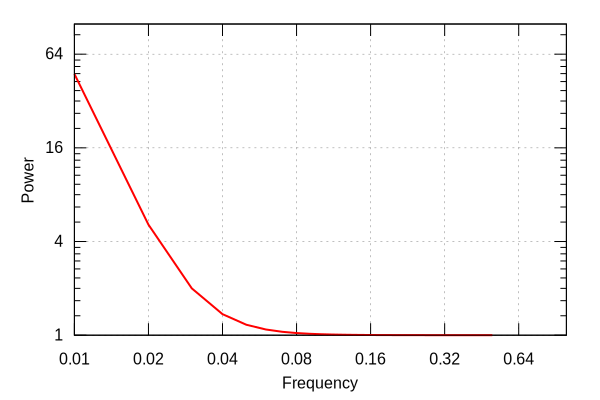
\includegraphics[width=\columnwidth]{subpix/ps.pdf}
	\caption{
		The noise model/inverse weights/inverse filter used in the subpixel
		bias demonstration in figures~\ref{fig:subpix-bias} and \ref{fig:subpix-noerr}.
		It is a simple Fourier-diagonal 1/f + white noise spectrum
		typical for ground-based CMB observations. The frequency axis is in
		dimensionless units in this toy example, but for real telescopes the
		transition from white noise is typically a few Hz, corresponding
		to multipoles of hundreds on the sky.
	}
	\label{fig:ps}
\end{figure}

Discontinuous residuals are not necessarily problematic. The trouble arises
when this is coupled with a likelihood\footnote{The equivalent for filter+bin is a filter that
impacts some modes more than others (which is the whole point of a filter),
and for destriping it's the baseline length and any amplitude priors.
} where some modes have much less weight than others. Ground-based CMB
telescopes suffer from atmospheric emission that acts as a large source
of noise on long timescales. This leads to time-ordered data noise power
spectra similar to the one sketched in figure~\ref{fig:ps}, with
a white noise floor at short timescales (high frequency) transitioning to a steep
rise of several orders of magnitude as one moves to longer timescales
(low frequency). In this case long-wavelength modes have orders of magnitude
lower weight in the likelihood than short-wavelength modes. Put another way,
they are orders of magnitude \emph{cheaper to sacrifice} when the model can't fully
fit the data.

\subsection{1D toy example}
To illustrate the interaction between a nearest neighbor pointing matrix's
subpixel errors and a likelihood where large scales have low weight, let
us consider a simple 1D case where 100 samples scan uniformly across 10 pixels:
\begin{lstlisting}
npix  = 10
nsamp = 100
pix   = np.arange(nsamp).astype(float)*npix/nsamp
\end{lstlisting}
A standard nearest-neighbor pointing matrix for this looks like:
\begin{lstlisting}
P = np.zeros((nsamp,npix))
for i, p in enumerate(pix):
	P[i,int(np.round(pix[i]))%npix] = 1
\end{lstlisting}
We assume a typical Fourier-diagonal ``1/f'' noise model
$N(f) = \big(1+(f/f_\text{knee})^\alpha\big)^{-1}$
with $f_\text{knee}=0.03$ and $\alpha=-3.5$, and bild the
inverse noise matrix/filter/baseline-prior $F$ by
projecting the inverse noise spectrum $N^{-1}$ into pixel space:
\begin{lstlisting}
freq   = np.fft.rfftfreq(nsamp)
inv_ps = 1/(1+(np.maximum(freq,freq[1]/2)/0.03)**-3.5)
F = np.zeros((nsamp,nsamp))
I = np.eye(nsamp)
for i in range(nsamp):
	F[:,i] = np.fft.irfft(inv_ps*np.fft.rfft(I[i]), n=nsamp)
\end{lstlisting}
The signal itself consists of just a long-wavelength sine wave:\footnote{
Since all the mapmaking methods we will discuss are linear,
signal and noise can analysed independently. Since the focus
in this example is bias, it's therefore enough to consider a
signal-only data set, and we thus don't add any noise.}
\begin{lstlisting}
signal = np.sin(2*np.pi*pix/npix)
\end{lstlisting}

With this in place, we can now define our map estimators.

\subsubsection{Binning}
The \emph{binned map} is simply the mean value of the samples
in each pixel, with no weighting:
\begin{lstlisting}
map_binned = np.linalg.solve((P.T.dot(P)), P.T.dot(signal))
\end{lstlisting}
This is the unweighted least-squares solution for the map.

\subsubsection{Maximum-likelihood}
The maximum-likelihood solution of equation~\ref{eq:model} for the
sky image $m$ is
\begin{align}
	\hat m = (P^TN^{-1}P)^{-1}P^TN^{-1}d
\end{align}
where $N$ is the covariance matrix of the noise $n$. This is the
generalized least-squares solution for the map.
In our toy example, $N^{-1} = F$, so the \emph{maximum-likelihood map}
is
\begin{lstlisting}
map_ml = np.linalg.solve((P.T.dot(F).dot(P)),P.T.dot(F.dot(signal)))
\end{lstlisting}

\subsubsection{Filter+bin}
As the name suggests, filter+bin consists of filtering the time-ordered
data, and then making a binned map. We'll use $F$ as our filter, so
the \emph{filter+bin map} is
\begin{lstlisting}
map_fb = np.linalg.solve(P.T.dot(P), P.T.dot(F).dot(signal))
\end{lstlisting}
The filter+bin map is biased by design, so to interpret or debias it one
needs to characterize this bias. There are two common approaches
to doing this: Observation matrix and simulations.

\paragraph{Observation matrix}
The observation matrix approach
recognizes that the whole chain of operations observe, filter, map
together make up a linear system, and can therefore be represented
as a matrix, called the \emph{observation matrix} \citep{bicep2-obsmat}.
Building this matrix is heavy, but doable for some
surveys. Under the standard assumption that the observation step is
given by equation~\ref{eq:model}, the observation matrix is given by
\begin{lstlisting}
obsmat = np.linalg.inv(P.T.dot(P)).dot(P.T.dot(F).dot(P))
\end{lstlisting}
and using it, we can define a debiased filter+bin map
\begin{lstlisting}
map_fb_deobs = np.linalg.solve(obsmat, map_fb)
\end{lstlisting}

\paragraph{Simulations}
Alternatively, and more commonly, one can characterize the bias
by simulating the observation of a set of random skies, passing
them through the filter+bin process, and comparing the properties
of the input and output images. The standard way of doing this is
by assuming that equation~\ref{eq:model} describes the observation
process, and that the bias can be described by a \emph{transfer function}:
a simple independent scaling of each fourier mode. Under
these assumptions, we can measure and correct the bias as follows.
\begin{lstlisting}
nsim = 1000
sim_ips = np.zeros(npix//2+1)
sim_ops = np.zeros(npix//2+1)
for i in range(nsim):
	sim_imap = np.random.standard_normal(npix)
	sim_omap = np.linalg.solve(P.T.dot(P), P.T.dot(F).dot(P).dot(sim_imap))
	sim_ips += np.abs(np.fft.rfft(sim_imap))**2
	sim_ops += np.abs(np.fft.rfft(sim_omap))**2
tf = (sim_ops/sim_ips)**0.5
map_fb_detrans = np.fft.irfft(np.fft.rfft(map_fb)/tf, n=npix)
\end{lstlisting}

\subsubsection{Destriping}
Destriping splits the noise into a correlated and uncorrelated part,
and models the correlated noise as as a series of slowly changing
degrees of freedom to be solved for jointly with the sky image itself
\citep{descart-destriper,planck-destriping}.
The data is modeled as
\begin{align}
	d &= Pm + Qa + n_w
\end{align}
where $n_w$ is the white noise with diagonal covariance matrix $N_w$,
and $Q$ describes how each correlated noise degree of freedom $a$
maps onto the time-ordered data, typically in the form of seconds
(ground) to minutes (space) long baselines. Given this, the
maximum-likelihood solutions for $a$ and $m$ are
\begin{align}
	Z &= I - P(P^TN_w^{-1}P)^{-1}P^TN_w^{-1} \notag \\
	a &= (Q^TN_w^{-1}ZQ + C_a^{-1})^{-1} Q^TN_w^{-1}Zd \notag \\
	m &= (P^TN_w^{-1}P)^{-1}P^TN_w^{-1}(d - Qa) \label{eq:destripe}
\end{align}
where $C_a$ is one's prior knowledge of the covariance of $a$.
Destriping allows a speed/optimality tradeoff in the choice of
baseline length and prior, and approaches the maximum likelihood
map when the baseline length is a single sample and $C_a + N_w = N$.
We implement this limit below, but explore other choices in section~\ref{sec:toy-2d}.
In our toy example $N_w = I$, so $C_a = F^{-1}-I$.
\begin{lstlisting}
iCa = np.linalg.inv(np.linalg.inv(F) - I)
Z   = I-P.dot(np.linalg.solve(P.T.dot(P), P.T))
a   = np.linalg.solve(Z+iCa, Z.dot(signal))
map_ds = np.linalg.solve(P.T.dot(P), P.T.dot(signal - a))
\end{lstlisting}

\subsubsection{Results}
\begin{figure}
	\centering
	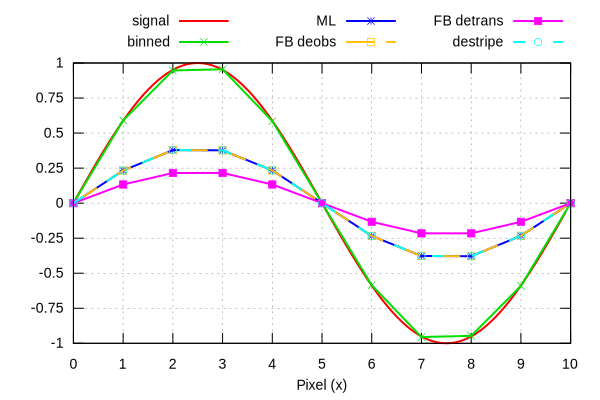
\includegraphics[width=\columnwidth]{subpix/model_error_toy.pdf}
	\caption{
		Demonstration of large loss of power in long-wavelength mode
		caused by the poor subpixel treatment in the standard nearest-neighbor pointing matrix.
		Figure~\ref{fig:ps} shows the noise model/inverse weights/inverse filter
		used in the various methods.
		\dfn{signal}: The input signal, a smooth long-wavelength mode,
		sampled at 10 samples per output pixel.
		\dfn{binned}: Simple binned map (the unweighted average per pixel).
		Very suboptimal in the presence of correlated noise, but unbiased.
		\dfn{ML}: Maximum-likelihood map. 2/3 of the signal amplitude is lost despite
		the naive expectation of biaslessness for this estimator.
		\dfn{FB deobs}: Filter+bin map debiased using an observation matrix.
		Identical to ML.
		\dfn{FB detrans}: Filter+bin map debiased by deconvolving a
		transfer function measured from simulations. Even more biased
		than the others due to ignoring mode coupling.
		\dfn{destripe}: Destriper in the maximum-likelihood limit
		(1-sample baselines with optimal baseline prior). Identical to ML.
	}
	\label{fig:subpix-bias}
\end{figure}

Figure~\ref{fig:subpix-bias} compares the recovered 1D sky ``images''
for the different mapmaking methods for this toy example. All methods
are expected to have a small loss of power at small scale (called
the ``pixel window'') due to averaging the signal within each pixel,
but this effect is well-known, easy to model, and not our focus here.
We deconvolve it using the following function before plotting.
\begin{lstlisting}
def dewin(x): return np.fft.irfft(np.fft.rfft(x)/np.sinc(freq),n=len(x)).real
\end{lstlisting}
After pixel window deconvolution the binned map (green) closely matches the
input signal (red). The same can not be said for the other estimators.
Maximum likelihood, filter+bin with observation matrix debiasing and destriping
(which are all equivalent in the limit I consider here) are strongly biased,
with the signal only being recovered with 1/3 of its real amplitude.

The situation is even worse for for filter+bin with simulation-based debiasing,
as this suffers from an additional bias due to assuming that the Fourier modes
are independent.\footnote{This additional bias disappears if the simulations
have exactly the same statistical properties as the real signal we wish to
recover.}

\subsubsection{Explanation}
To see why inaccuracies in modelling the signal at sub-pixel scales can bias
the largest scales in the map, let us consider the example in figure~\ref{fig:nearest-neigh},
where a detector measures a smooth, large-scale signal while moving across a few
pixels. With a nearest-neighbor pointing matrix it is impossible to model this
smooth signal: the model for each sample is simply that of the closest pixel,
regardless of where inside that pixel it is. The model therefore looks like
a staircase-like function in time domain.

Given that we can't exactly match the signal, what is the best approximation?
Let us consider two very different alterantives. \dfn{Model A}: The value in each pixel
is the average of the samples that hits it, making the model curve trace the
smooth signal as closely as it can. This is the green curve in figure~\ref{fig:nearest-neigh},
and has the sawtooth-like residual shown with the blue curve. It is probably the
model most people would choose if asked to draw one manually.
\dfn{Model B}: The value in each pixel is zero, and the residual is simply the signal itself.
Model B seems like a terrible fit to the data, but under a reasonable noise model
for a ground-based telescope, like the one shown in figure~\ref{fig:ps}, it
will actually have a higher likelihood (lower $\chi^2 = r^TN^{-1}r$
where $r$ is the residual) than model A. The reason is that while model B has a much
larger residual than model A, model B's residual is smooth and hence has most of its
power at low frequency in time domain where $N^{-1}$ is very small. Meanwhile, model A's
residual extends to all frequencies due to its jagged nature, including the costly high
frequencies. The actual maximum-likelihood solution will be intermediate between these
two cases, sacrificing some but not all of the large-scale power in the model to make
the residual smoother.

\begin{figure}
	\centering
	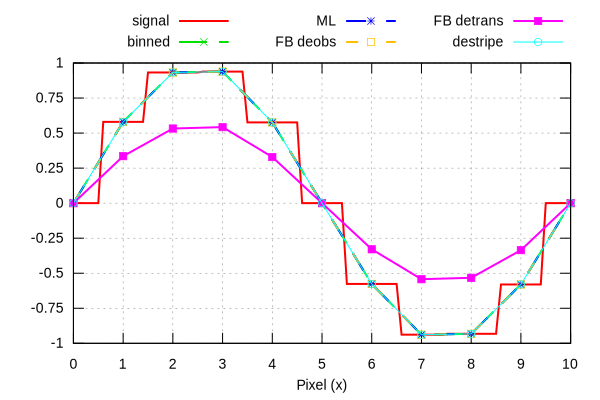
\includegraphics[width=\columnwidth]{subpix/model_error_toy_noerr.pdf}
	\caption{
		Like figure~\ref{fig:subpix-bias}, but with the input signal
		having the same nearest-neighbor pixelization as the models.
		In this case all models except FB detrans are unbiased.
	}
	\label{fig:subpix-noerr}
\end{figure}

To demonstrate that the bias really is caused by subpixel errors,
I repeated the simulation with a signal that follows the same nearest-neighbor
behavior as the data model, thus eliminating subpixel errors. The
result is shown in figure~\ref{fig:subpix-noerr}. The bias has disappeared
in all methods except filter+bin with transfer-function based debiasing,
which has an additional source of bias due to its assumption of a Fourier-diagonal
filter response.

\subsection{2D toy example}
\label{sec:toy-2d}
The 1D toy example is useful for understanding the origin of the bias, but
its unrealistic observing pattern makes it insufficient for exploring
optimality/bias tradeoffs in the different methods. I therefore made a larger
toy example where a single detector scans at constant speed across a square
patch, sampling $N_\text{scan} = 400$ equi-spaced rows with $N_\text{scan}$
equi-spaced samples per row, followed by a column-wise scan the same patch,
leading to a total cross-linked data set $N_\text{samp} = 2 N_\text{scan}^2 = 3200$
samples long. This equi-spaced grid of samples was chosen to make it easy to
simulate a signal directly onto the the samples without needing the complication
of pixel-to-sample projection. These samples will then be mapped onto a
square grid of pixels with a side length of $N_\text{side} = 100$ using
the different mapmaking methods.

For the signal I draw realizations from a CMB-like $1/l^2$ power spectrum
with a Gaussian beam with standard deviation $\sigma=3$ pixels. Here $l$
is the pixel-space wave-number, which I evaluate in the higher
resolution sample space as
\begin{lstlisting}
ly = np.fft.fftfreq(N_scan)[:,None] * N_side/N_scan
lx = np.fft.fftfreq(N_scan)[None,:] * N_side/N_scan
l  = (ly**2+lx**2)**0.5
\end{lstlisting}
With this I can define the signal power spectrum $C_l = l^{-2}$ and beam $B_l = \exp(-l^2 \sigma^2/2)$,
and draw signal realizations as
\begin{lstlisting}
signal_map = np.fft.ifft2(np.fft.fft2(np.random.standard_normal((N_scan,N_scan)))*Cl**0.5*Bl).real
signal_tod = np.concatenate([signal_map.reshape(-1), signal_map.T.reshape(-1)])
\end{lstlisting}
The last step here takes into account that the simulated scanning pattern covers the
field twice, first horizontally and then vertically.

For the noise I use a simple 1/f spectum $N(f) = 1 + (f/f_\text{knee})^\alpha$,
with \lstinline{f = np.fft.rfftfreq(N_samp)}
and the knee frequency $f_\text{knee}$ corresponding to 1/30th of the side length,
$f_\text{knee} = 0.5\cdot 30/N_\text{scan} = 0.0375$ (6.7 pixel wavelength), and with
an atmosphere-like exponent $\alpha=-3.5$.

The pixel coordinates of each sample are
\begin{lstlisting}
pix_pat1 = (np.mgrid[:N_scan,:N_scan]*N_side/N_scan).reshape(2,-1)
pix_pat2 = pix_pat1[::-1]
pix = np.concatenate([pix_pat1,pix_pat2],1)
\end{lstlisting}
which I use to build the nearest-neighbor pointing matrix
\begin{lstlisting}
iy, ix = np.floor(pix).astype(int)%N_side
P_nn   = scipy.sparse.csr_array((np.full(N_samp,1),(np.arange(N_samp),iy*N_side+ix)),shape=(N_samp,N_pix))
\end{lstlisting}

\begin{figure*}[p]
	\centering
	\begin{closetabcols}
		\begin{tabular}{C{13mm}ccm{1mm}ccC{14mm}}
			& Signal & Noise & & Noise & Signal & \\
		Input &
		\includegraphics[width=30mm,valign=m]{subpix/toy2d_input_signal_map.png} &
		& &
		\includegraphics[width=30mm,valign=m]{subpix/toy2d_binned_nn_noise_map.png} &
		\includegraphics[width=30mm,valign=m]{subpix/toy2d_binned_nn_signal_map.png} &
		bin \\[13.6mm]
		ML &
		\includegraphics[width=30mm,valign=m]{subpix/toy2d_ml_nn_signal_map.png} &
		\includegraphics[width=30mm,valign=m]{subpix/toy2d_ml_nn_noise_map.png} & &
		\includegraphics[width=30mm,valign=m]{subpix/toy2d_destripe_plain_004_nn_noise_map.png} &
		\includegraphics[width=30mm,valign=m]{subpix/toy2d_destripe_plain_004_nn_signal_map.png} &
		\vc{DS 4}\\[13.6mm]
		\vc{ML w1}&
		\includegraphics[width=30mm,valign=m]{subpix/toy2d_ml_cap_1_nn_signal_map.png} &
		\includegraphics[width=30mm,valign=m]{subpix/toy2d_ml_cap_1_nn_noise_map.png} & &
		\includegraphics[width=30mm,valign=m]{subpix/toy2d_destripe_prior_004_nn_noise_map.png} &
		\includegraphics[width=30mm,valign=m]{subpix/toy2d_destripe_prior_004_nn_signal_map.png} &
		\vc{DS+ 4}\\[13.6mm]
		\vc{ML w2}&
		\includegraphics[width=30mm,valign=m]{subpix/toy2d_ml_cap_2_nn_signal_map.png} &
		\includegraphics[width=30mm,valign=m]{subpix/toy2d_ml_cap_2_nn_noise_map.png} & &
		\includegraphics[width=30mm,valign=m]{subpix/toy2d_destripe_plain_064_nn_noise_map.png} &
		\includegraphics[width=30mm,valign=m]{subpix/toy2d_destripe_plain_064_nn_signal_map.png} &
		\vc{DS 64}\\[13.6mm]
		\vc{ML w3}&
		\includegraphics[width=30mm,valign=m]{subpix/toy2d_ml_cap_3_nn_signal_map.png} &
		\includegraphics[width=30mm,valign=m]{subpix/toy2d_ml_cap_3_nn_noise_map.png} & &
		\includegraphics[width=30mm,valign=m]{subpix/toy2d_destripe_prior_064_nn_noise_map.png} &
		\includegraphics[width=30mm,valign=m]{subpix/toy2d_destripe_prior_064_nn_signal_map.png} &
		\vc{DS+ 64}\\[13.6mm]
		\vc{ML lin} &
		\includegraphics[width=30mm,valign=m]{subpix/toy2d_ml_lin_signal_map.png} &
		\includegraphics[width=30mm,valign=m]{subpix/toy2d_ml_lin_noise_map.png} & &
		\includegraphics[width=30mm,valign=m]{subpix/toy2d_destripe_prior_004_lin_noise_map.png} &
		\includegraphics[width=30mm,valign=m]{subpix/toy2d_destripe_prior_004_lin_signal_map.png} &
		\vc{DS+ 4 lin}
	\end{tabular}
	\end{closetabcols}
	\caption{
		Example signal and noise maps for the different mapmaking methods.
		The top left map is the input signal, which is directly evaluated
		at 4x higher resolution than what is used for reconstructing the output maps.
		All output maps were built built from the same data and assume a nearest neighbor pointing matrix,
		except for the last row where a bilinear pointing matrix was used.
		The color range is the same for all panels.
		The binned map (top right) is bias-free but has uselessly high noise. Maximum likelihood (ML)
		and destriping with short baselengths (with (DS+) and without (DS) baseline amplitude prior,
		which only matters for the shortest baseline)
		are all low-noise but biased on large scales. This bias goes away as the noise model
		is artificially whitened (ML w$X$) or the baseline length is increased (for destriping),
		but this comes at a cost of increased noise on all scales.
		Bilinear mapmaking (last row) instead avoids the bias by eliminating most of the model error.
		It can be difficult to judge how significant the bias and noise levels are from
		these images. See figures~\ref{fig:2d-bias} and \ref{fig:2d-noise} for easier to
		interpret comparisons of the signal and noise power spectra respectively.
	}
	\label{fig:2d-maps}
\end{figure*}

\begin{figure}
	\centering
	\hspace*{-5mm}\includegraphics[width=1.10\columnwidth]{subpix/model_error_toy_2d.pdf}
	\caption{
		Comparison of the subpixel bias of different mapmaking methods
		described in section~\ref{sec:2d-cases} and discussed in section~\ref{sec:2d-results}.
		Standard maximum-likelihood (thick blue) is strongly biased, as are all but
		the (very noisy) longest destriping baseline. This bias disappears (ML)
		or is greatly reduced (DS) when switching to bilinear interpolation in the pointing matrix.
		See figure~\ref{fig:2d-noise} for the corresponding noise spectra.
		The wavenumber $l$ is dimensionless and with a Nyquist frequency of 0.5.
		I interpret upturn at $l>0.4$ as aliasing, which
		is expected and not relevant for the biases we consider here.
	}
	\label{fig:2d-bias}
\end{figure}

\begin{figure}[h!]
	\centering
	\hspace*{-5mm}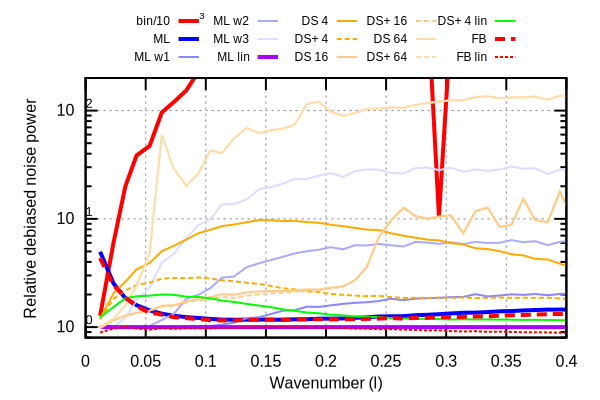
\includegraphics[width=1.10\columnwidth]{subpix/model_error_toy_2d_noise.pdf}
	\caption{
		Comparison of the optimality for the methods defined in section~\ref{sec:2d-cases}, measured
		as the debiased noise power spectrum (using the bias measurements from figure~\ref{fig:2d-bias})
		for each method relative to that of bilinear maximum-likelihood mapmaking.
		Note the logarithmic vertical axis, and that binned case was divided by $10^3$
		to bring it partially inside the plot bounds.
		The wavenumber $l$ is dimensionless and with a Nyquist frequency of 0.5.
		It's clear that simple bias mitigation
		methods like artificially whitening the noise model or increasing the
		baseline length are too costly to be practical.
	}
	\label{fig:2d-noise}
\end{figure}

\subsubsection{Cases}
\label{sec:2d-cases}
I will investigate 5 classes of nearest-neighbor maps:
\begin{enumerate}
	\item \dfn{bin}: Simple binned map, which I expect to be unbiased but very noisy
	\item \dfn{ML}: Maximum-likelihood map. Ideally unbiased and optimal, but will deviate
		from this due to model errors.
	\item \dfn{ML w$X$}: Maximum-likelihood maps with a ``whitened'' noise model,
		which overestimates the
		white noise power by a factor $10^X$, $X\in\{1,2,3\}$, reducing the overall
		correlatedness of the noise model. I expect the bias to be proportional to the
		overall dynamic range of the noise model,
		so making the nosie model whiter should reduce bias. The cost will be suboptimal noise
		weighting, leading to a noisier map, but it might be worth it.
	\item \dfn{DS $X$}: Destriping map with a baseline of $X\in \{4,16,64\}$ samples and no amplitude
		prior. This is probably the most common type of destriping. The baseline lengths
		can be compared with the noise knee wavelength of 6.7 pixels $\approx$ 27 samples.
		This is the wavelength where the correlated and white noise powers are equal.
	\item \dfn{DS+ $X$}: Like DS $X$, but uses the correlated part of the maximum-likelihood
		noise model as an amplitude prior ($C_a$ in equation~\ref{eq:destripe}).
	\item \dfn{FB}: Filter+bin mapmaking where a transfer function is measured using
		simulations based on the data model, and this is deconvolved when measuring
		the power spectrum. This is the standard approach for filter+bin mapmaking.
		In this case only the power spectrum is debiased, not the map, so I don't
		show an example map for this case.
\end{enumerate}

Since all the mapmaking methods are linear, the signal and noise can be mapped separately.
I make 400 signal-only and noise-only data realizations, and map them using each method,
computing the mean signal and noise power spectra.

\subsubsection{Results}
\label{sec:2d-results}
Example maps are shown in figure~\ref{fig:2d-maps},
while the bias and noise are quantified in figures~\ref{fig:2d-bias} and \ref{fig:2d-noise}
respectively.
As expected the binned map is unbiased but extremely noisy. The maximum-likelihood
map is low-noise, but measurably biased on all scales, with a power deficit of
a few percent at the smallest scales which grows to almost 100\% on the largest scales.
The deficit appears to fall proportionally with the whitening, with ML w1 and w2
being respectively 10x and 100x as close to unbiased. Sadly this comes at the cost of
40\% and 350\% higher noise power respectively. These numbers may differ for real-world
cases, but this still seems like a very expensive bias mitigation method.
All but the longest-baseline destriped maps are also strongly biased,
with the shortest baseline being considerably worse than ML for almost all scales.
Much like we saw with the ML variants, the less biased destriping versions
come at a high cost in noise. Finally, the filter+bin map is biased even after simulation-based
debiasing due to the simulations not capturing the subpixel behavior of the real data.
Both the bias and noise levels are the same as maximum-likelihood in this example.

To test whether the observed biases are truly caused by subpixel errors, I repeat
the simulations with only one sample per pixel ($N_\text{scan} = N_\text{side}$).
As expected this results in an unbiased power spectrum for all methods.\footnote{
	Even filter+bin, which ignores mode coupling, ends up having an unbiased power
	spectrum because the simulations used to build the transfer function followed
	the same distribution as the real signal.
}

\subsubsection{Effective mitigation of subpixel errors}
There will be no subpixel errors in the limit of infinitely small pixels,
so it's tempting to simply reduce the pixel size to solve the problem. This
does work, but since subpixel errors are proportional to $|\nabla s \cdot \vec \Delta|$,
where $s$ is the true, smooth signal on the sky and $\vec \Delta = [\Delta_x,\Delta_y]$
is the pixel shape, the improvement is only first order in the pixel side length.
A much more feasible solution is to instead improve the subpixel handling in the
pointing matrix. Going from nearest neighbor to bilinear interpolation is enough
to practically eliminate subpixel errors without reducing pixel size. We can
implement this in the toy example by defining
\begin{lstlisting}
pix_left = np.floor(pix).astype(int)
ry, rx  = pix-pix_left
iy1,ix1 = pix_left % N_side
iy2,ix2 = (pix_left+1)% N_side
weights = np.concatenate([
		(1-ry)*(1-rx), (1-ry)*rx,
		ry    *(1-rx), ry    *rx])
samps   = np.tile(np.arange(N_samp),4)
inds    = np.concatenate([
	iy1*N_side+ix1, iy1*N_side+ix2,
	iy2*N_side+ix1, iy2*N_side+ix2])
P_lin = scipy.sparse.csr_array((weights,(samps,inds)),shape=(N_samp,N_pix))
\end{lstlisting}
Bilinear mapmaking results in a different pixel window than
the standard \lstinline{pixwin_nn = sinc(ly)[:,None]*sinc(lx)[None,:]}
of nearest neighbor mapmaking. I measure this empirically using simulations
of simple binned mapmaking, and find it to have the separable form
\lstinline{pixwin_lin = linwin1d(ly)[:,None]*linwin1d(lx)[None,:]},
with \lstinline{linwin1d} being plotted in figure~\ref{fig:linwin1d}.

\begin{figure}
	\centering
	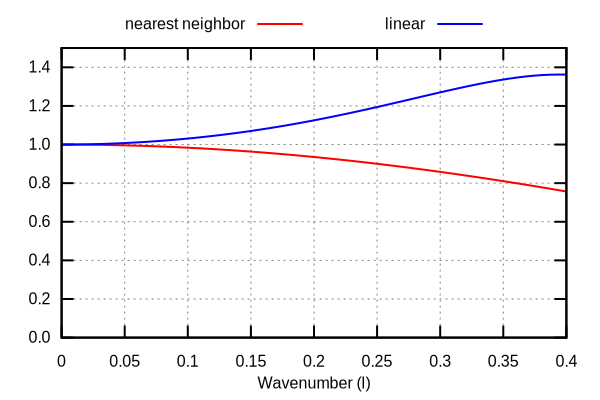
\includegraphics[width=\columnwidth]{subpix/tfun_lin_1d.pdf}
	\caption{Comparison of the 1D pixel window for nearest neighbor
	mapmaking (red, $\text{sinc}(l)$) and linear mapmaking (blue). The 2D pixel window
	is the outer product of the 1D one along each axis. The pixel
	windows model the response of the Fourier coefficients to
	binned (unweighted) mapmaking. Square it to get the effect on
	the power spectrum.}
	\label{fig:linwin1d}
\end{figure}

Since each sample in bilinear mapmaking gets contributions from the four closest pixels,
the pointing matrix is about four times slower than the standard nearest neighbor
version. However, as shown in figures~\ref{fig:2d-bias} and \ref{fig:2d-noise}
this cost is worh it, with bilinear maximum-likelihood mapmaking being bias-free
and even lower noise than standard ML. The bias is also greatly reduced for
destriping, but not eliminated.

\section{Don't think you're safe just because you avoid subpixel errors}
By no means all model errors have the strong impact on large scales
that subpixel errors do. For example, gain errors typically have a
scale-independent response while pointing errors broaden the beam, damping
small scales but not large ones. It is, in fact, quite difficult to come up
with other mechanisms by which model errors can cause large-scale power
bias. One example I found requires a multi-detector system with large
gain error error differences between the detectors, combined with a noise model where the noise is
dominated by a long-wavelength common mode (strong correlation between detectors
at long wavelengths). This is implemented in the program \verb|common_mode_test.py|
(see section~\ref{sec:code})
with the output shown in figure~\ref{fig:common}. In this example the
large scales are biased \emph{high} and also subject to a phase shift, while
the small scales have negligible bias.

\begin{figure}
	\centering
	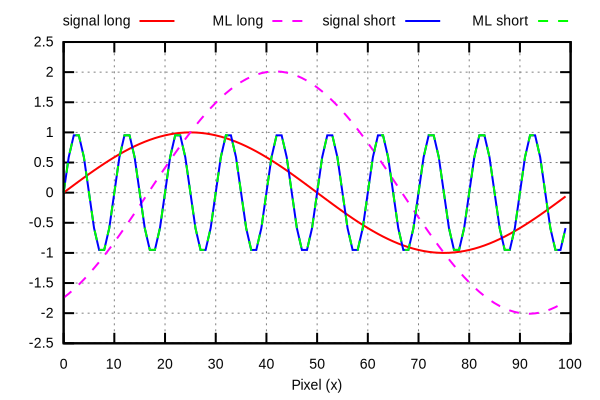
\includegraphics[width=\columnwidth]{common_mode/common.pdf}
	\caption{
		Demonstration of large-scale bias in a multi-detector system
		due to an interaction between strong large-scale
		detector correlations in the noise model and large
		relative gain errors between the detectors.
		\dfn{signal long}: An input long-wavelength signal,
		with the same pixelization as the output to avoid subpixel bias.
		\dfn{ML long}: Corresponding maximum-likelihood map, which
		exhibits both an amplitude and phase error.
		\dfn{signal short} and \dfn{ML short}: The same, but for a
		short-wavelength mode. Here the bias is negligible,
		despite the model's gain errors being scale-independent.
	}
	\label{fig:common}
\end{figure}

While the commmon-mode/bias-interplay works as a demonstration, it is a much
less robust error mechanism than subpixel errors, and requires quite extreme
parameters to produce appreciable bias. In my tests it also tends to disappear
as more data is added and crosslinking increases, and I have not been able to
provoke large-scale bias using this method for full-scale realistic datasets
(unlike subpixel errors!).

It would be convenient if the difficulty in finding model error mechanisms that
bias large scales meant that subpixel errors are the only ones one needs to
worry about, but sadly that does not seem to be the case. In my practical
experience with ground-based CMB mapmaking there have been cases of large-scale
power loss where subpixel errors were responsible for less than half of the
total bias. In these cases the difficulty in finding these mechanisms becomes
a curse rather than a blessing, since it makes it very difficult to track down
the source of the bias.

What makes model error bias especially insidious is that
it is completely invisible to any simulation that does not explicitly include
that particular type of model error. For example, a simulation where the CMB
is read off from a simulated map using the same pointing matrix as is used
in the mapmaking itself would be blind to subpixel errors. Given the many
possible ways the real data might deviate from one's model of it, it is hard
to be sure that one has included all the relevant types of model error in the simulations.
It is therefore very easy to trick oneself into believing that one has an
unbiased analysis pipeline while there are in fact $\mathcal{O}(1)$ biases remaining.

\section{Useful tests}
The unintuitive large-scale effects of model errors rely on the interaction
between model errors and non-local weighting/filtering. A noise model (or filter) with
a large dynamic range, such as one capturing the huge ratio between the long-wavelength
and short-wavelength noise power for ground-based CMB telescopes, is therefore
much more vulnerable to large-scale power loss than one appropriate for a
space-based telescopes which have almost flat noise power spectra. This suggests
the following tests for large-scale model error bias:
\begin{enumerate}
	\item Compare power spectra with those from a space-based telescope.
		This is reliable but comes at the cost of being able to make an independent measurement.
	\item Split the data into subsets with different ratios of correlated noise to white noise
		and check their consistency. This could for example be a split by the
		level of precipitable water-vapour (PWV) in the atmosphere. High-PWV-data
		would be expected to have a higher dynamic range and therefore be more vulnerable.
	\item Map the same data both using the standard noise model/filter and a
		less optimal one an artificially reduced lower dynamic range, e.g. one that
		underestimates the amount of correlated noise. The latter should result in
		less a biased but noisier map, as we saw in figures~\ref{fig:2d-bias} and \ref{fig:2d-noise}.
		If the maps are consistent, then large-scale model error bias is probably not an issue.
\end{enumerate}

\section{Source code}
\label{sec:code}
The source code and data files behind these examples is available at
\url{https://github.com/amaurea/model_error2}. The 1D and 2D subpixel
simulations are available in \verb|subpix/model_error_toy.py| and \verb|subpix/model_error_toy.py|
respectively, while the common-mode/gain-error interplay example is in
\verb|common_mode/common_mode_test.py|.

\section{Conclusion}

\begin{enumerate}
	\item \textbf{All CMB current mapmaking methods are vulnerable to model error bias},
		including maximum-likelihood mapmaking, destriping and filter+bin mapmaking.
	\item \textbf{The most common model error is subpixel errors} due to the assumption that
		the signal is constant inside each pixel (a nearest-neighbor pointing matrix),
		but \textbf{other types of model error can also be important}.
	\item Model error bias can manifest in unintuitive ways, with a common symptom
		being a large ($\mathcal{O}(1)$) \textbf{loss of long-wavelength power} in the maps.
	\item The size of the bias is proportional to the dynamic range of the filter/noise model.
		Hence it is \textbf{important for ground-based measurements of the unpolarized CMB}
		due to the presence of large-scale atmospheric noise there, but is \textbf{much less
		important for polarization measurements or space-based telescopes}.
	\item \textbf{Simulations are blind to these biases unless specifically designed to
		target them}. There is a large risk of ending up thinking one has an unbiased
		pipeline despite there being large bias in the actual CMB maps.
	\item An effective way of testing for this bias is to \textbf{also map the data using a
		(much) lower dynamic range noise model/filter}\footnote{Or much longer baselines for destriping}
		and checking if this leads to consistent power spectra.
\end{enumerate}

\section*{Acknowledgements}
I would like to thank Jon Sievers for first making me aware
that subpixel errors weren't just limited to X'es around point
sources and other small-scale effects.
My work is supported by a grant from Simons Foundation.

\bibliographystyle{act_titles}
\bibliography{refs}

\end{document}
